\documentclass[12pt]{article}

\usepackage{amsmath}
\usepackage[polish]{babel}
\usepackage[utf8]{inputenc}
\usepackage[T1]{fontenc}
\usepackage{fancyhdr}
\usepackage{tikz}
\usepackage{graphicx}
\graphicspath{ {./images/} }

\usepackage{hyperref}
\hypersetup{
    colorlinks=true,
    linkcolor=black,
    filecolor=blue,      
    urlcolor=blue
}

\title{Drzewa binarne: BST oraz AVL}

\author{Eryk Andrzejewski - 145277}

\pagestyle{fancy}
\fancyhf{}
\fancyhead[L]{\leftmark}
\fancyhead[R]{\thepage}

\begin{document}
    \maketitle
    \tableofcontents
    \newpage
    
    \section{Wstęp}
        Tematyką niniejszego sprawozdania są dwie struktury danych, będące drzewami binarnymi: drzewo BST (z angielskiego \textit{Binary Search Tree} - drzewo binarnych poszukiwań) oraz drzewo AVL (nazwa jest syntezą inicjałów autorów: Gieorgija Adelsona-Wielskiego i Jewgienija Łandisa).
        
        Drzewa te składają się z węzłów. Każdy węzeł może mieć maksymalnie dwoje dzieci. Węzły identyfikowane są poprzez wartości, które zawierają - nazywane są one również \texit{kluczami}.
        
        \subsection{Drzewo BST}
            Drzewo BST jest takim drzewem binarnym, w którym lewe poddrzewo każdego węzła zawiera elementy wyłącznie mniejsze od wartości w tym węźle, a prawe poddrzewo zawiera elementy nie mniejsze od niego.
            
            Możliwe oczywiście są różne wariacje takiej struktury danych. W mojej implementacji założyłem, że wszystkie klucze są różne. Założenie to jest o tyle istotne, że klucze wykorzystuję do identyfikacji poszczególnych węzłów. Gdyby nie były one unikatowe, pojawiłby się problem chociażby podczas usuwania węzła - nie byłoby jednoznaczne, który element ma zostać usunięty.
            
            Drzewo BST jest stosunkowo nieskomplikowaną strukturą danych. Jej przewagą w stosunku do zwyczajnej listy (która jednak jest nieco prostsza w implementacji), jest to, że w optymistycznym przypadku operacje, takie jak wyszukiwanie elementów w drzewie, czy wstawianie ich do drzewa, mają złożoność obliczeniową $O(\log{n})$, zamiast złożoności $O(n)$.
            
            Drzewo BST cieszy się pewną przewagą, w stosunku do listy, ale nie jest pozbawione wad. Operacja wstawiania odpowiednio spreparowanych danych przyczynia się do tego, że drzewo degeneruje się do listy. Przykładowo, możemy wstawić do drzewa posortowane już (rosnąco lub malejąco) liczby. W takim przypadku drzewo przyjmie postać posortowanej listy. W tym momencie drzewo BST traci wiele ze swoich cennych zalet.
            
            Antidotum na ten problem może być algorytm DSW, który służy do równoważenia drzewa. Po jego wykonaniu, nawet z drzewa o strukturze listy, otrzymamy zrównoważone drzewo (rozpatrując wszystkie różne gałęzie, łączące korzeń z jednym z liści, to różnica długości między najkrótszą i najdłuższą taką gałęzią, będzie wynosiła maksymalnie jeden). Jednak to programista musi zadbać, by w odpowiednim momencie ten algorytm wywoływać.
            
            Alternatywą dla powyższego rozwiązania jest drzewo AVL.
            
        \subsection{Drzewo AVL}
            Drzewo AVL jest nadal drzewem BST, jednak jest ulepszone o pewien drobny szczegół - każdy węzeł posiada dodatkowe pole zwane współczynnikiem balansu (w skrócie \texit{BF}, z ang. \texit{Balance Factor}). Jest on równy różnicy wysokości lewego i prawego podrzewa. Drzewo AVL dopuszcza tylko trzy stany, odpowiadające trzem różnym wartościom BF: -1, 0 oraz 1.
            
            Jakakolwiek inna wartość BF oznacza, że drzewo ma niepoprawną strukturę. Aby je \texit{naprawić}, stosuje się rotacje. Są ich cztery rodzaje i zależnie od struktury węzła i jego dzieci, wybiera się odpowiednią z nich.
            
            Dzięki zastosowaniu takiego rozwiązania mamy pewność, że drzewo będzie zawsze zrównoważone (jest ono naprawiane, w razie potrzeby, po każdej operacji, która modyfikuje jego strukturę - np. po wstawieniu nowego elementu, albo usunięciu jakiegoś węzła).
            
            Odbywa się to niestety kosztem tego, że drzewo AVL jest nieco bardziej skomplikowane w działaniu i w implementacji. Po wstawieniu/usunięciu węzła, należy aktualizować pole współczynnika balansu w węzłach nadrzędnych (rodzicu, dziadku, pradziadku itd.). W nich również może zajść potrzeba wykonania rotacji przywracającej poprawną strukturę drzewa.
            
            Uważam jednak, że stosowanie drzew AVL jest bardzo opłacalne. Dlaczego? 
            
            Pierwszym argumentem jest oczywiście średnia wydajność - pozbywamy się przypadku pesymistycznego, który jest zmorą oryginalnego drzewa BST.
            
            Należy jeszcze wspomnieć o czymś równie istotnym, co ujawnia się przy rekurencyjnej implementacji drzewa BST. Jeżeli drzewo będzie miało zbyt dużą wysokość, rekurencyjne przechodzenie z węzła do węzła może skończyć się przepełnieniem stosu. I to jest poważny problem, który należy w jakiś sposób rozwiązać - z jednej strony chroniąc program przed nieoczekiwanym przerwaniem działania, z drugiej strony również przed atakami, które mogą wykorzystywać tę podatność (podatności z gatunku buffer overflow mogą wydawać się niegroźne, ale jest wręcz przeciwnie - atakujący może pokusić się o przygotowanie odpowiedniego shellcode i wstrzyknąć kod maszynowy, i na przykład przez nadpisanie adresu powrotu przejąć kontrolę nad maszyną). Należy dbać o wszystkie błędy dotyczące pamięci, jeżeli mamy zamiar napisać kod produkcyjny - w przypadku kodów pisanych w zamiarach czysto-edukacyjnych, z których raczej nikt poza nami nie będzie korzystał, nie ma takiej potrzeby.
            
            Aby wyeliminować ten problem, można pokusić się o wyeliminowanie rekurencji (co też zdarzyło mi się zrobić w przypadku niektórych implementacji, np. w przypadku algorytmu DSW), albo po prostu skorzystać z drzewa AVL, w którego przypadku przepełnienie stosu nie będzie miało miejsca (jest to technicznie niemożliwe, dane musiałyby osiągać \textit{kosmiczne} rozmiary).
            
            Istnieje również trzecia możliwość, którą zastosowałem samemu podczas testów - skorzystać z API systemu operacyjnego i poprosić go o przyznanie stosu o większym rozmiarze. Nie jestem pewien, na ile byłoby to dobre rozwiązanie dla oprogramowania produkcyjnego, ale do testowania wydajności algorytmów powinno być idealne. Skrajnie, poprosiłem nawet o przydzielenie gibibajta pamięci jako stos.
            \newpage
            
    \section{Testy wydajnościowe}
        Zarówno drzewo BST, jak i drzewo AVL zaimplementowałem w języku C++. Implementacja jest obiektowa, skorzystać z tych struktur danych można przy pomocy odpowiednich klas: \texttt{BinarySearchTree} oraz \texttt{AvlTree}.
        
        Z klas tych korzysta prosty program testujący \texit{trees}, który na podstawie argumentów, z jakimi się go uruchamia, wykonuje odpowiednią operację: tworzy drzewo, wyszukuje w nim najmniejszy element, bądź też wypisuje wszystkie metodą in-order. Program ten w wyniku wypisuje czas działania na standardowe wyjście, o czym za chwilę powiem więcej.
        
        Powyższy program testowany jest przy użyciu konfigurowalnego skryptu \textit{benchmark}, z który przygotowałem podczas pracy nad pierwszym sprawozdaniem i postanowiłem go wykorzystać również tym razem. Generuje on zestawy danych o odpowiednim rozmiarze i rozkładzie (pozwala więc wygenerować np. sto tysięcy zupełnie losowych liczb, albo pięćdziesiąt tysięcy liczb posortowanych malejąco). Po wygenerowaniu uruchamia testowany program.
        
        W zależności od konfiguracji, czas wykonania jest mierzony przez skrypt testujący, albo program poddawany testom. Jest to mała innowacja w stosunku do wersji skryptu \textit{benchmark} stosowanej przy okazji pierwszego sprawozdania. Wprowadzenie możliwości wykonywania pomiarów przez testowany program umożliwia uzyskanie rzetelnych wyników - dzięki temu jestem w stanie zmierzyć wyłącznie czas wykonywania się określonego algorytmu przeszukującego/równoważącego drzewo, a operacje takie jak tworzenie drzewa, czy jego destrukcja nie są brane pod uwagę podczas pomiaru czasu.
        
        Wynikiem testów jest plik JSON, który następnie jest przetwarzany przez skrypt \textit{plotter}, który z kolei rysuje wykresy wydajności.
        
        W poniższych podrozdziałach prezentował będę wyniki poszczególnych testów, wraz z ich krótkimi omówieniami. Dodam jeszcze tylko, że wszystkie testy odbywają się na rozkładzie malejącym, czyli ciągu postaci $(n, n-1, n-2,..., 1)$. Rozkład ten ma na celu wyeksponowanie wad drzewa BST i zestawienie ich z zaletami drzewa AVL. Rozmiary danych, dla których testowano różne operacje, mogą się różnić - były one dobierane empirycznie, tak by wykres podkreślał złożoność obliczeniową algorytmu.
        \newpage
        
        \subsection{Tworzenie drzewa}
        Tak prezentują się wykresy czasów tworzenia drzew: BST oraz AVL, w zależności od ilości wstawianych węzłów:
        \begin{figure}[h]
            \centering
            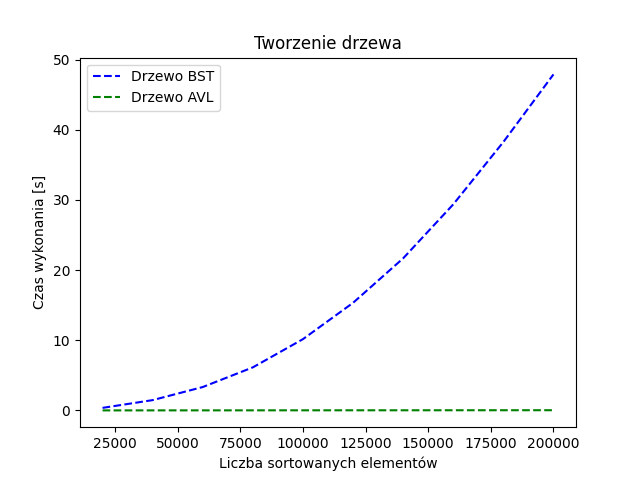
\includegraphics[width=\textwidth]{wykresy/Tworzenie_drzewa.png}
        \end{figure}
        
        Jak można zauważyć, czas tworzenia drzewa AVL jest zdecydowanie krótszy, niż w przypadku drzewa BST - jest wręcz niezauważalny. Jest to spowodowane tym, że obydwa drzewa testowane są na danych posortowanych malejąco. Drzewo AVL jest na takie dane odporne i zawsze pozostaje zrównoważone, a drzewo BST nie - w jego przypadku tworzy się struktura, która bardziej przypomina listę, niż drzewo. Wobec tego, aby wstawić kolejny element (który jest mniejszy od wszystkich poprzednich), trzeba przeiterować po wszystkich istniejących już węzłach.
        
        Operacja wstawiania posortowanej malejąco listy do drzewa BST będzie miała więc złożoność obliczeniową rzędu $O(n^2)$, natomiast w przypadku drzewa AVL będzie to złożoność rzędu $O(n\log{n})$ - drzewo to jest zawsze zrównoważone, więc dla $n$ elementów w drzewie, które będziemy wstawiali, jego wysokość będzie rzędu $\log{n}$.
        
        Dodam jeszcze tylko, że testowana przeze mnie implementacja była rekurencyjna.
        
        \subsection{Szukanie elementu minimalnego}
        Tak prezentuje się wykres czasu wyszukiwania najmniejszego elementu, od wielkości danych:
        \begin{figure}[h]
            \centering
            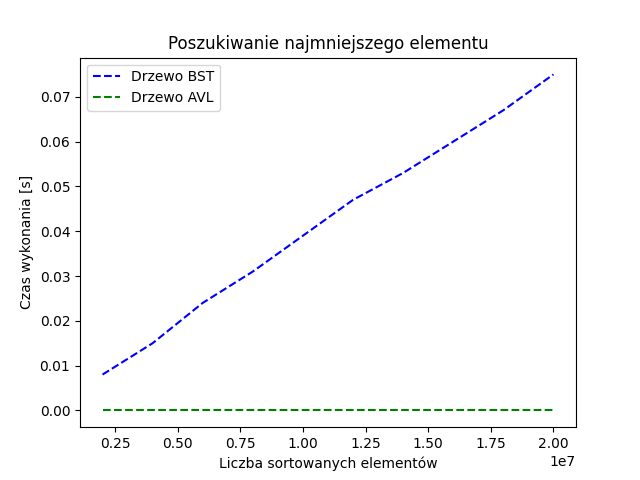
\includegraphics[width=\textwidth]{wykresy/Poszukiwanie_najmniejszego_elementu.png}
        \end{figure}
        
        Z racji, że drzewa testujemy na danych posortowanych malejąco, to w przypadku drzewa BST trzeba będzie przeiterować przez wszystkie węzły, aby dostać się do węzła z najmniejszym kluczem. Złożoność obliczeniowa takiej operacji to $O(n)$. W przypadku drzewa AVL ponownie jest lepiej, bo jest ono zrównoważone, więc złożoność takiej operacji to $O(\log{n})$. Tutaj ponownie wygrywa AVL. Jego wykres jest ponownie praktycznie niezauważalny, ale nic na to nie poradzę. Żeby jakikolwiek wzrost był widoczny, musiałbym prezentować wyłącznie wykres dla drzewa AVL (złożoność obliczeniowa drzewa BST jest większa, więc wykres narasta szybciej, a jego skalowanie upraszcza wykres drzewa AVL do prostej), albo też testować obydwa algorytmy dla bardzo małej ilości danych, ale takie testy byłyby niemiarodajne i podatne na zakłócenia.
        
        Algorytmy poszukiwania najmniejszego elementu zostały zaimplementowane przeze mnie zarówno rekurencyjnie, jak i iteracyjnie. Implementacja iteracyjna jest wyjątkowo prosta i powinna być minimalnie wydajniejsza niż rekurencyjna (składa się z tylko jednej, prostej pętli), dlatego też ją wykorzystałem do testów.
        \newpage
        
        \subsection{Przeszukiwanie drzewa metodą in-order}
        Przeszukiwanie drzewa metodą in-order wymaga dostania się do każdego węzła, jaki znajduje się w drzewie i wypisania jego klucza, oczywiście dzieje się to wszystko w odpowiedniej kolejności. W tym przypadku jednak drzewo AVL nie powinno mieć przewagi w stosunku do drzewa BST (chyba, że chodzi o wyeliminowanie problemu przepełnienia stosu na wskutek zbyt dużej ilości rekurencyjnych wywołań). Złożoność obliczeniowa tej operacji będzie podobna dla obu drzew - jest rzędu $O(n)$.
        
        \begin{figure}[h]
            \centering
            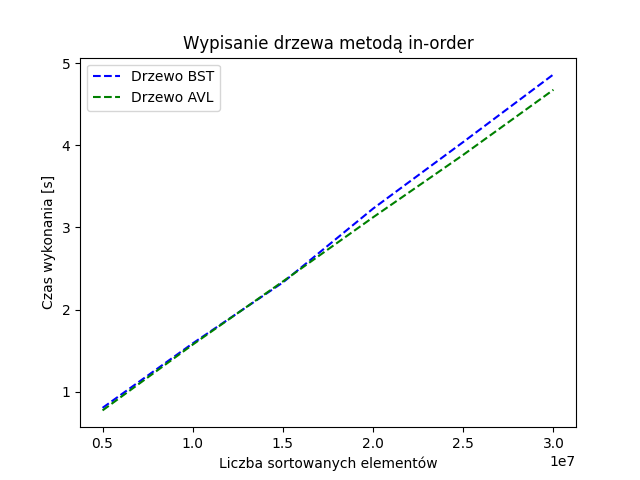
\includegraphics[width=\textwidth]{wykresy/Wypisanie_drzewa_metodą_in-order.png}
        \end{figure}
        
        Występują oczywiście jakieś nieduże różnice, ale zdecydowanie bliżej tym wykresom do siebie, niż w poprzednich testach.
        
        \newpage
        
        \subsection{Algorytm DSW}
        Algorytm ten służy do równoważenia drzewa BST. W skrajnym przypadku, z listy, jaką otrzymamy po wstawieniu elementów posortowanych malejąco, jest w stanie stworzyć strukturę, która znacznie bardziej przypomina drzewo - i jest zrównoważona.
        
        Teoretycznie można by się pokusić o implementację tego algorytmu również w przypadku drzewa AVL - trzeba byłoby wtedy zadbać również o aktualizację współczynnika balansu i ewentualne rotacje. Jednak wydaje mi się to być pozbawione sensu, ponieważ drzewo AVL jest już i tak zawsze zbalansowane.
        
        Wobec tego, zgodnie z poleceniem, na poniższym wykresie znajduje tylko jedna krzywa, określająca czas wykonania się tego algorytmu dla drzewa BST, w zależności od rozmiaru danych wejściowych.
        
        Algorytm DSW ma złożoność obliczeniową rzędu $O(n)$. Wykres zdaje się to potwierdzać.
        
        \begin{figure}[h]
            \centering
            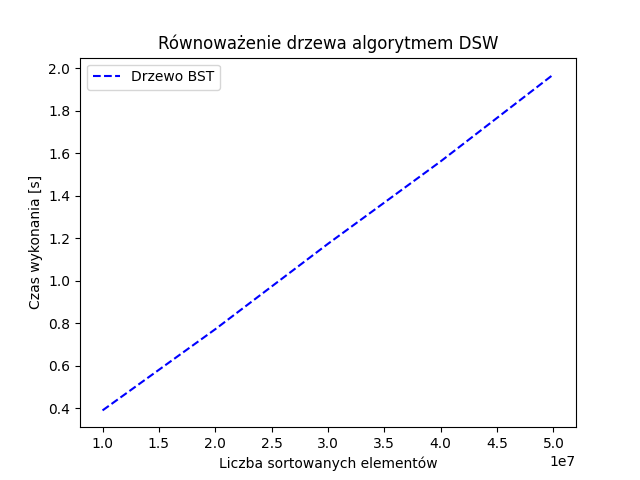
\includegraphics[width=\textwidth]{wykresy/Równoważenie_drzewa_algorytmem_DSW.png}
        \end{figure}
        
        Jak widać, musiałem użyć niemałych rozmiarów danych (50 milionów elementów), aby krzywa (a właściwie prosta) złożoności obliczeniowej była wyraźnie widoczna. Mimo tak dużych rozmiarów danych, czasy wykonania są nadal całkiem małe. Świadczy to o dużej wydajności tego algorytmu.
        
    \section{Podsumowanie}
        Uważam, że drzewo AVL jest generalnie dobrą inwestycją - owszem, trzeba poświęcić nieco czasu aby je dobrze zaimplementować (choć można również wykorzystywać gotowe implementacje, które już zostały porządnie przetestowane), ale pozbawione jest najgorszych wad drzewa BST.
        
        Ale, jak to często w informatyce bywa, nie ma jednej odpowiedzi na pytanie - którego drzewa powinienem użyć. Trzeba więc dobierać strukturę danych odpowiednio do zastosowań.
    
\end{document}
